\documentclass{beamer}
\usepackage[utf8]{inputenc}

\hypersetup{
    colorlinks,%
    citecolor=blue,%
    filecolor=blue,%
    linkcolor=blue,%
    urlcolor=blue 
    %urlcolor=mygreylink     % can put red here to better visualize the links
}

\author[Sowmya Vajjala]{Instructor: Sowmya Vajjala}

\title[LING 520]{LING 520: Computational Analysis of English}
\subtitle{Semester: FALL '16}

\date{20 September 2016}

\institute{Iowa State University, USA}
%%%%%%%%%%%%%%%%%%%%%%%%%%%

\begin{document}

\begin{frame}\titlepage
\end{frame}

\begin{frame}
\frametitle{AACL Conference and Workshops - Comments}
\begin{itemize}
\item How did the R workshop go? What did you learn? \pause
\item How many people in the class are RegEx gurus now? \pause
\item Any interesting language processing related talks at AACL? \pause
\item Reg Assignment 2: Deadline is on 27th, but do not wait until 26th midnight to ask me for support.
\end{itemize}
\end{frame}

\begin{frame}
\frametitle{Morphological Parsing}
\begin{itemize}
\item What is it?: taking in a word and showing its morphological structure as output. \pause
\item Examples: 
\begin{tabular}{c|c}
input & output \\
\hline
cars & car + Noun + Plural \\
caught & catch + Verb + Past \\
caught & catch + Verb + PastPart \\
he & he + pronoun + 3rdPerson + Singular \\
\end{tabular}
\end{itemize}
\end{frame}

\begin{frame}
\frametitle{More complex language example}
Morphological parsing output for Estonian.
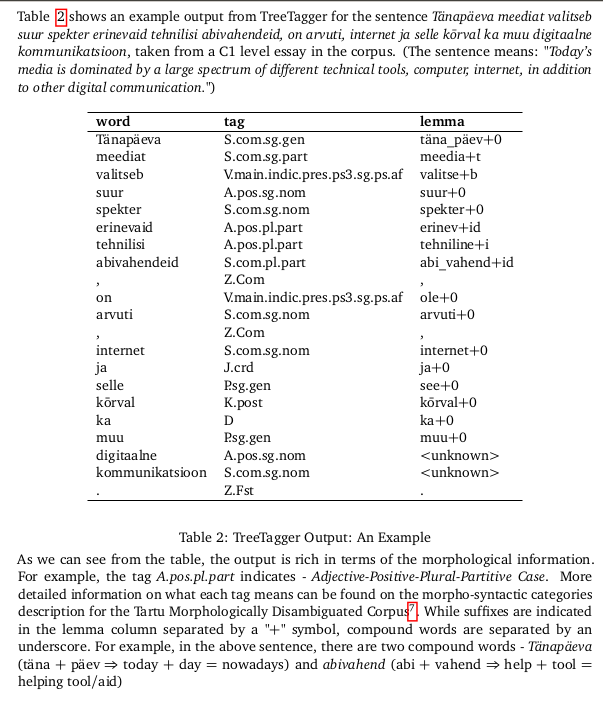
\includegraphics[width=0.7\textwidth]{morphparsingexample.png}
\end{frame}

\begin{frame}
\frametitle{Why get such details?}
\begin{itemize}
\item Useful to capture spelling variations of words for doing search, especially for morphologically rich languages with lot of inflections.
\item Useful to develop good POS taggers and parsers for such languages.
\item Useful for creating large dictionaries for spell checking (using edit distance, for example)
\item Useful in machine translation, to choose the right translation of a word.
\item Useful for speech processing applications as well.
\end{itemize}
\end{frame}

\begin{frame}
\frametitle{How do we do morphological parsing?}
\begin{itemize}
\item Language is productive. Some suffixes can be applied to each and every noun or verb or some other class.
\item Hence, it is not possible to list all possible forms for all possible words in a language (even in a language without a lot of inflections). 
\item Solution 1: Copiously create a large set of rules and then write a program implementing those rules.
\item Solution 2: Ask linguists to create such parses for a lot of data, and write a program that "learns" the rules based on all those examples.
\item Two forms of morphological parsing we discuss today: stemming, lemmatization
\end{itemize}
\end{frame}

\begin{frame}
\frametitle{Stemming}
\begin{itemize}
\item In some applications, we don't need a full morphological parse, but we only need a way to group orthographically similar words. 
\item This can be done by just stripping off word endings using a set of rules. This is called stemming.
\item Porter Stemmer is a popular stemming algorithm for English. Originally proposed by Martin Porter in 1980 
\item There are other stemmers available, and there are stemmers for other languages.
\end{itemize}
\end{frame}

\begin{frame}
\frametitle{Porter Stemmer}
\begin{itemize}
\item Rules: from Original 1980 paper \url{http://tartarus.org/~martin/PorterStemmer/def.txt}
\item NLTK implementation: \url{http://www.nltk.org/_modules/nltk/stem/porter.html}
\item Note: PorterStemmer just dumbly follows those rules. It does not maintain a lexicon or anything. So, even if you enter a proper name, it stems it. 
\item In some NLP applications, such limitations do not create any new issues.
\end{itemize}
\end{frame}

\begin{frame}
\frametitle{Lemmatization}
\begin{itemize}
\item In some other NLP tasks, grouping words that are from the same root, although they have different surface forms is also important (e.g., goose and geese won't be recognised as one by a stemmer).
\item To get the root of a given word, we need to perform lemmatization. 
\item Lemma of "was" is "be", but stem will be was. Lemma of "believes" is "belief". But stem will be "believ".
\end{itemize}
\end{frame}

\begin{frame}
\frametitle{Lemmatization: How does it work?}
\begin{enumerate}
\item What resources do we need?
\begin{itemize}
\item Lists of irregular words and their morphological forms for each POS tag category.
\item Suffix stripping rules like stemming, along with POS tag of the word.
\end{itemize}
\item For a given word and POS combo, first we look at the list of irregular words for that POS. If the word does not exist in this list, we move to the rules part.
\end{enumerate}
\end{frame}

\begin{frame}
\frametitle{Lemmatization in NLTK}
\begin{itemize}
\item in NLTK, it uses "Wordnet" to perform lemmatization.
\item Wordnet (\url{http://wordnet.princeton.edu/}) is much more than a lemmatizer, but has a utility called "Morphy" which does the morphological processing NLTK uses for lemmatization.
\item Some information on Morphy: \url{https://wordnet.princeton.edu/man/morphy.7WN.html}
\item NLTK code: Morphy function definition in \url{http://www.nltk.org/_modules/nltk/corpus/reader/wordnet.html}
\end{itemize}
\end{frame}

\begin{frame}
\frametitle{Practice Exercise}
Form into groups of three, and do the following:
\begin{enumerate}
\item There is a .txt file on Blackboard, showing how to load various NLTK stemmers and use them.
\item Prepare a test suite of 10 words or so, and study the differences between the outputs of these stemmers. 
\item Study the use of WordNetLemmatizer, and how the output varies for the same word based on the POS tag you choose. Test with a few words.
\item If you finish these, find out what other languages does NLTK support for stemming and lemmatizing.
\end{enumerate}
Spend about 20 minutes in doing this exercise, and in the remaining time, give a quick summary of what you discovered.
\end{frame}

\begin{frame}
\frametitle{Bonus Exercises for Enthusiasts}
\begin{itemize}
\item Learn to use RegExpStemmer in NLTK.
\item Start working on Problem Set 3.
\end{itemize}
\end{frame}
\end{document}

